\documentclass{article}
\usepackage{amsmath,amsfonts,amssymb,graphicx,color}
\begin{document}
\section*{\small 2.3 Periodogram}
Time series, independently of the phenomenon they represent, are generally presented in the time domain. Another interesting view of the same series is in the frequency domain, considering that any stationary time series can be expressed as a combination of sinusoidal functions, thanks to the Fourier transform. The frequency domain tool used by time series analysts is called spectrum, and its representation is called periodogram. It is possible to obtain it as follows:
\begin{equation}
y_t = \sum\limits_{i=1}^{\frac{n}{2}}[\beta_{1_{i}}\cos(2\pi\omega_{i}t) + \beta_{2_{i}}\sin(2\pi\omega_{i}t)]
\end{equation}
The $\beta$'s work as regression parameters, obtained from: $\beta_{1_{i}}=A_{i} \cos(\phi_{i})$ and $\beta_{2_{i}}=-A \sin(\phi_{i})$, where $\phi$ is called the phase; it determines the starting point (in degrees) for the cosine wave. A is the amplitude.
\\The spectral analysis investigates the frequency domain representation of the series to determine how important cycles of different frequencies are in accounting for the behaviour of \textit{y$_t$}. Therefore, the periodogram is useful to identify the dominant periods (or frequencies) of a time series. Peaks in a periodogram indicate frequencies of cyclical movements with a certain periodicity. The periodicity \textit{P} of a phenomenon is related to its frequency $\omega$: $P=2 \pi / \omega$. It means that for a monthly series, seasonal frequencies are $\pi/6$, $\pi/3$, $\pi/2$, $2\pi/3$, $5\pi/6$ and $\pi$, and they correspond to 1, 2, 3, 4, 5 and 6 cycles per year (for quarterly sampled series, the two seasonal frequencies are $\pi/2$; one cycle per year, and $\pi$; two cycles per year).\\The trading day frequency is 0.348, since a daily component which repeats every seven days goes through 4.348 cycles in a month of average length 30.4375 days. It means, then, that 0.348 is the trading days frequency for monthly sampled time series, considering the average length of a year (365.25 days). Actually, the original trading days frequency (4.348) is higher than the Nyquist frequency. {\color{red} If any signal has a frequency higher than the $\omega_{N_{yq}}$, it is an aliasing signal, i.e. it is indistinguishable from a lower-frequency signal. So, there is the need for filter this high-frequencies signals with a so called lowpass filter. In this way, the signal “appears” with much lower $\omega$. In this case, $\omega=4.348$ appears as 0.348.}\\A time series with a strong seasonal component should have peaks at the seasonal frequencies, while a seasonally adjusted time series should not have any peaks at those frequencies. Moreover, the presence of the trend component is always evidenced by a peak at frequency zero and so, when a periodogram has high values at low frequencies, it means that the long-term component (the trend) is dominating the series. On the contrary, if high values of the periodogram concentrate more at high frequencies, the time series is rather trendless and has a significant irregular component.\\JDemetra+ contains different spectral diagnostics. First, it is possibile to have a spectral plot of the raw time series, obtained (by default) after a first difference operation to get the data stationary. Indeed, non-stationarity of the series could lead to a misinterpretation of the periodogram.  One other issue is related to the presence of outliers, since they can influence the interpretation of the periodogram as well. This is why a pre-transformation of data is advisable, as done by both TRAMO/SEATS and X-13-ARIMA.  As is visible from figure 3, in JDemetra+ the seasonal frequencies are marked as grey vertical lines, while the violet lines represents the trading day frequency.\\
\begin{figure}[h!]
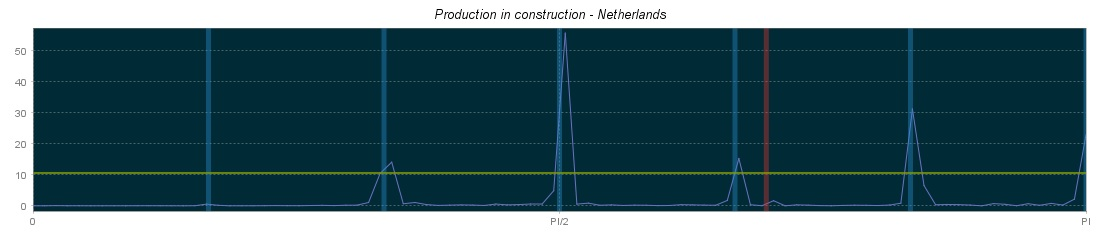
\includegraphics[width=\linewidth]{raw.jpg}
\caption{\textbf{\small Figure 3: JDemetra+ representation of a periodogram}}
\end{figure}
\\In addition to the ‘raw’ periodogram, once the seasonal adjustment procedure has been carried out, JDemetra+ offers some spectral diagnostics. In particular, it is possible to check periodograms of the seasonally adjusted series, residuals and irregular component. Further details will be given in the next chapter.
\end{document}